\documentclass[11pt]{article}

\usepackage[margin=1in]{geometry}
\usepackage{mathtools,amssymb,amsthm}
\usepackage{microtype}
\usepackage{booktabs}
\usepackage{enumitem}
\usepackage{hyperref}
\usepackage{graphicx}
\usepackage{tikz}
\usetikzlibrary{positioning}
\usepackage{fancyhdr}

\title{Canonical Structural Analysis:\\
A Deterministic Compilation Framework for Workload-Relative Dependency Analysis}
\author{Jose Luna}
\date{\today}

\newtheorem{definition}{Definition}
\newtheorem{theorem}{Theorem}
\newtheorem{lemma}{Lemma}
\newtheorem{proposition}{Proposition}
\newtheorem{corollary}{Corollary}

% Proof-audit helper: explicitly list prerequisites for each theorem.
\newcommand{\deps}[1]{\par\noindent\textbf{Dependencies.} #1\par}

\begin{document}

\maketitle

% Running header
\pagestyle{fancy}
\fancyhead[L]{Canonical Structural Analysis}
\fancyhead[R]{Luna}
\fancyfoot[C]{\thepage}
\renewcommand{\headrulewidth}{0.4pt}
\renewcommand{\footrulewidth}{0pt}

\begin{abstract}
Paper 1 formalized dependency as a workload-relative property computed on a directed graph by deletion and reachability. This paper addresses the prior compilation question: what exactly is the graph on which that predicate operates?
We define canonical structural analysis as a deterministic compilation framework that maps heterogeneous system descriptions into canonical typed structural objects. The framework separates domain extraction, normalization, canonicalization, workload projection, and reachability-graph construction. Rather than identifying any existing representation as universal, the paper treats compiler IRs, dependence graphs, provenance models, workflow graphs, and canonical graph representations as ingredients in a broader structural compilation model.
The central object is a canonical structural object from which workload-specific directed graphs can be projected for dependency analysis. The contribution is not a new graph theory or a replacement for compiler theory. It is a formal interface between concrete systems and workload-relative dependency predicates, designed to make analysis deterministic, representation-independent, and suitable for later analyses such as dependency, resilience, redundancy, and governance.
\end{abstract}
\section{Introduction}
\label{sec:introduction}
% [Audit: No citation needed] Original research narrative and problem statement.
Paper 1 defined a workload-relative dependency predicate on a directed graph, evaluated by counterfactual deletion and reachability. It did not define how that graph is obtained from a concrete system. This paper fills that gap.

% [Audit: No citation needed] Clarifying question and manuscript contribution.
The central question is:
\[
\text{What exactly is } G?
\]
We answer by defining a deterministic \emph{structural} pipeline that maps heterogeneous system descriptions into a canonical structural object, and then projects that object into the workload-specific graph required by the dependency predicate.

% [Audit: Citation optional] Figure pointer for reader orientation.
Figure~\ref{fig:pipeline-overview} previews the end-to-end interface: concrete systems enter on the left, and Paper~1's dependency analysis consumes the projected reachability graph on the right.

% [Audit: No citation needed] Paper~1 bridge (series coherence).
\paragraph{A missing bridge (Paper~1 vs.\ this paper).}
Paper~1 assumes the existence of an analysis graph $G$ on which deletion and reachability are evaluated. The purpose of this paper is to construct that object: given a concrete system description $d$, we define a deterministic compilation function $C_\chi$ that produces the workload-class graph $G_\chi$ (and the induced workload anchors) as an explicit, representation-independent artifact.

\begin{figure}[t]
  \centering
  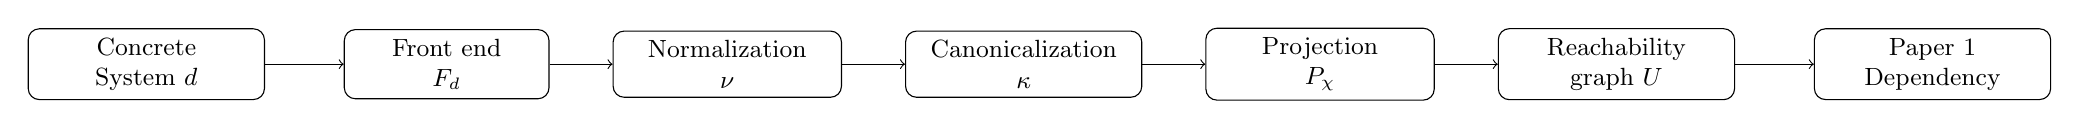
\begin{tikzpicture}[node distance=6mm, every node/.style={font=\small}]
    \node[draw, rounded corners, align=center, minimum width=3.0cm] (sys) {Concrete\\System $d$};
    \node[draw, rounded corners, align=center, right=10mm of sys, minimum width=2.6cm] (fe) {Front end\\$F_d$};
    \node[draw, rounded corners, align=center, right=8mm of fe, minimum width=2.9cm] (norm) {Normalization\\$\nu$};
    \node[draw, rounded corners, align=center, right=8mm of norm, minimum width=3.0cm] (canon) {Canonicalization\\$\kappa$};
    \node[draw, rounded corners, align=center, right=8mm of canon, minimum width=2.9cm] (proj) {Projection\\$P_\chi$};
    \node[draw, rounded corners, align=center, right=8mm of proj, minimum width=3.0cm] (reach) {Reachability\\graph $U$};
    \node[draw, rounded corners, align=center, right=10mm of reach, minimum width=3.0cm] (p1) {Paper 1\\Dependency};

    \draw[->] (sys) -- (fe);
    \draw[->] (fe) -- (norm);
    \draw[->] (norm) -- (canon);
    \draw[->] (canon) -- (proj);
    \draw[->] (proj) -- (reach);
    \draw[->] (reach) -- (p1);
  \end{tikzpicture}
  \caption{Overall compilation pipeline connecting concrete systems to the workload-relative dependency predicate of Paper~1.}
  \label{fig:pipeline-overview}
\end{figure}

\section{Motivation}
\label{sec:motivation}
% [Audit: Citation required] Claims about existing system/graph artifacts across communities.
\paragraph{Problem.}
Heterogeneous systems are increasingly analyzed with graph-based tools, but each domain exposes different structural artifacts: compiler IRs and program graphs for software \cite{llvmLangRef,mlirDoc}, workflow and provenance graphs for data systems \cite{w3cprov,deelman2009}, and typed knowledge graphs for organizational and socio-technical structure \cite{hogan2021}. As a result, ``the graph'' used in downstream dependency reasoning is often implicit, ad hoc, or tightly coupled to a particular representation.

% [Audit: Citation required] Claims about what existing representations do (and do not) provide.
\paragraph{Gap.}
Existing IRs, code property graphs, provenance models, and workflow graphs preserve useful structure \cite{llvmLangRef,mlirDoc,yamaguchi2014cpg,w3cprov,deelman2009}, but none defines a deterministic \emph{cross-domain compilation contract} into the exact directed graph required by workload-relative dependency analysis. In particular, representation artifacts (naming, ordering, encoding choices) can leak into the analysis unless canonicalization and workload-class projection are made explicit.

\paragraph{Framework.}
As illustrated in Figure~\ref{fig:pipeline-overview}, Canonical Structural Analysis defines a deterministic structural compiler
\[
C_\chi = U \circ P_\chi \circ \kappa \circ \nu \circ F_d
\]
as the pipeline from a concrete system description to a workload-specific reachability graph. Extraction $F_d$ and normalization $\nu$ recover domain structure; canonicalization $\kappa$ erases representation artifacts; projection $P_\chi$ selects the information required by a workload class $\chi$; and $U$ constructs the directed graph consumed by the dependency predicate of Paper~1.

\paragraph{Contributions.}
\begin{enumerate}[label=(\arabic*),leftmargin=*]
  \item Defines the canonical structural object $\Sigma$.
  \item Defines a deterministic compilation function $C_\chi$.
  \item Proves determinism, idempotence, projection closure, representation invariance, workload preservation, compiler correctness, and minimal sufficiency.
  \item Separates compilation cost from query cost.
\end{enumerate}

\section{Related Work}
\label{sec:related-work}
This paper is positioned between compiler intermediate representations, program analysis graphs, code property graphs, provenance/workflow models, and canonical graph representations. Rather than proposing a new IR, we treat these bodies of work as established sources of structural information and as motivation for a compilation contract that (i) is deterministic, (ii) explicitly removes representation artifacts via canonicalization, and (iii) produces workload-class projections tailored to the dependency predicate of Paper~1.

\subsection{Compiler intermediate representations (LLVM, MLIR, IR design)}
Compiler intermediate representations provide a long-standing template for separating front-end extraction from optimization and analysis. LLVM IR is a widely used low-level IR with a stable specification and an ecosystem of analyses and transforms \cite{llvmLangRef}. More broadly, IR design emphasizes invariants, well-defined transformations, and analysis-friendly forms \cite{muchnick1997}.

MLIR extends this lineage by making heterogeneity explicit: multiple dialects can coexist, and lowering can proceed in stages while preserving enough structure for progressively different analyses \cite{mlirDoc}. This staged approach aligns with our separation of extraction and normalization from subsequent canonicalization and projection.

\emph{Stage mapping.} In the language of the structural compiler, LLVM/MLIR primarily inform $F_d$ (how to extract structure from concrete artifacts) and $\nu$ (how to normalize into analysis-friendly forms). They can also provide concrete substrates for $H$ when the domain is software, but they do not fix a domain-independent $\kappa$ or a workload-class projection contract $P_\chi$.

\emph{Contribution and gap relative to this framework.} IRs (LLVM/MLIR) contribute a principled pipeline view and concrete realizations of $F_d$ and $\nu$. They do not, by themselves, define a canonical representative across representation-equivalent compilations, nor do they make workload-relative projection and representation invariance explicit as part of the analysis interface. Our framework is designed to be \emph{implemented using} existing IR infrastructures when the source domain is software, while remaining applicable to non-compiler domains.

\subsection{Program analysis graphs (CFG, SSA, dominators, PDG, slicing)}
Graph representations are foundational in program analysis. Control-flow graphs (CFGs) and dominator trees support reachability and dominance reasoning in flowgraphs \cite{lengauer1979}. Static single assignment (SSA) form provides an analysis-friendly representation of def--use structure and enables many classic optimizations \cite{cytron1991}. Dependence graphs, and in particular the program dependence graph (PDG), make control and data dependences explicit and support optimizations and program understanding \cite{ferrante1987}. Program slicing further operationalizes dependency-like questions by computing the subset of program elements relevant to a slicing criterion \cite{weiser1981}.

These representations highlight two themes that motivate our pipeline. First, multiple graph views can be extracted from a single underlying artifact, depending on the analysis goal. Second, the correctness of downstream reasoning depends on the invariants guaranteed by earlier compilation stages.

\emph{Stage mapping.} These analyses contribute most directly to $P_\chi$ and $U$: they motivate the idea that a workload class should induce a projection to a particular relation family (e.g., control, data, dominance) and that many queries reduce to reachability computations on an analysis graph. In our terms, CFG/SSA/PDG structure can either live inside $H$ as typed edges or be produced by $P_\chi$ from a richer $H$, after which $U$ constructs the directed reachability graph consumed by Paper~1.

\emph{Contribution and gap relative to this framework.} Program analysis graphs contribute well-studied edge semantics and a vocabulary for workload-driven projection. They typically assume a code-centric source domain and do not provide a representation-invariance layer for comparing dependency answers across alternative front ends, optimization pipelines, or non-program systems. Our framework retains their graph-theoretic strengths while making $\kappa$, $P_\chi$, and $U$ explicit components of a deterministic compilation contract.

\subsection{Code property graphs and security-oriented unified representations}
Code property graphs (CPGs) unify syntactic (AST), control-flow, and dependence information into a single, queryable graph that supports scalable vulnerability discovery \cite{yamaguchi2014cpg}. The CPG line of work demonstrates that unifying multiple relation families can improve analysis ergonomics, especially when paired with graph query languages and domain-specific traversals.

\emph{Stage mapping.} CPGs contribute most naturally to the \emph{structural graph model} $H$: they exemplify a typed attributed graph that integrates multiple relation families. Operationally, CPG construction can be viewed as part of $F_d$ (extraction) and $\nu$ (normalization) for software domains, while vulnerability queries correspond to workload-like projections $P_\chi$ and reachability-style computations after $U$.

\emph{Contribution and gap relative to this framework.} CPGs contribute a practical demonstration of multi-relation unification and workload-like querying in security contexts. They do not directly address how to compile heterogeneous \emph{non-code} systems into a canonical structural object, nor do they formalize a canonicalization step $\kappa$ that factors out representation artifacts across multiple upstream encodings. In our setting, a CPG is best viewed as one possible realization of $H$ for software, with $\kappa$ and $P_\chi$ making the representation- and workload-interface explicit.

\subsection{Provenance models, workflow graphs, and knowledge graph structure}
Provenance and workflow models provide canonical examples of non-compiler domains in which dependency-like questions are central. The W3C PROV family standardizes entities, activities, agents, and derivation/usage relations \cite{w3cprov}. In database and data-management communities, provenance has also been formalized as a mechanism for explaining outputs in terms of inputs and transformations \cite{buneman2001,cheney2009}. Scientific workflow systems and DAG-based schedulers similarly treat computation as a graph of tasks and artifacts, supporting reproducibility, debugging, and what-if reasoning \cite{deelman2009}.

Knowledge graph research (RDF-style graphs, property graphs, and schema/ontology layers) further motivates typed attributed graph models in which vertices and edges carry semantic types and metadata \cite{hogan2021}.

\emph{Stage mapping.} These literatures contribute primarily to $H$ (a typed, attributed structural representation) and, implicitly, to $\mathcal W$ (workload spaces expressed as explanation, lineage, and what-if questions). Concretely, many provenance/workflow systems already materialize graphs that can serve as $H$ after normalization $\nu$; our framework adds an explicit $\kappa$ to remove representation artifacts and a workload-class projection $P_\chi$ that targets the specific reachability graph required by the dependency predicate.

\emph{Contribution and gap relative to this framework.} Provenance/workflow/knowledge-graph literatures contribute rich typed relation vocabularies outside of compilers and emphasize explainability and reproducibility. They typically do not provide a general-purpose canonicalization operator with explicit representation invariance guarantees, nor a dependency-specific projection contract aimed at producing the directed analysis graph used in Paper~1. Our framework serves as a compilation interface that can ingest these models into a canonical structural object suitable for uniform workload-relative dependency analysis.

\subsection{Canonical graph representations, canonical labeling, and isomorphism}
Canonicalization is closely related to canonical labeling and graph isomorphism. Practical toolchains (e.g., nauty/Traces) compute canonical labelings that can be used to obtain stable representatives under isomorphism for many graph families \cite{mckay2014}. Complexity-theoretic results on graph isomorphism also inform the limits of what a ``fully'' representation-invariant canonicalizer could guarantee in worst cases \cite{babai2016}.

In software and data systems, lighter-weight canonicalization is common: stable serializations, sorting by deterministic keys, and normalization of naming/addressing conventions often suffice to erase incidental artifacts without solving full isomorphism.

\emph{Stage mapping.} This body of work contributes directly to $\kappa$: it provides candidate algorithms and complexity bounds for choosing canonical representatives under a chosen equivalence. However, it does not specify which equivalence is appropriate for a domain, nor how canonicalization should interact with workload projection $P_\chi$.

\emph{Contribution and gap relative to this framework.} Canonical labeling and isomorphism contribute the mathematical grounding for strong forms of representation invariance. They do not determine which equivalences are semantically appropriate for a given domain or workload. Our framework keeps $\kappa$ abstract to allow domain-appropriate choices (from stable serialization to stronger canonical labeling) while still requiring determinism and proving properties (idempotence, invariance) at the level of the compilation contract.

Table~\ref{tab:related-work-map} summarizes how the major prior literatures align with the stages of the structural compiler.

\begin{table}[t]
\centering
\begin{tabular}{@{}lll@{}}
\toprule
Prior work & Contributes to & Gap addressed here \\
\midrule
LLVM/MLIR & $F_d,\nu$ & no cross-domain canonical object \\
PDG/CFG/SSA & $P_\chi,U$ & code-specific analysis graphs \\
CPG & $H$ & code-centric structural schema \\
PROV/workflows & $H,\mathcal W$ & no dependency-specific projection \\
Graph canonicalization & $\kappa$ & no domain/workload semantics \\
\bottomrule
\end{tabular}
\caption{How prior work maps to the canonical structural compiler.}
\label{tab:related-work-map}
\end{table}

Figure~\ref{fig:canonical-object} summarizes the three-part decomposition of the canonical structural object, and Figure~\ref{fig:compilation-stages} summarizes the stage structure of the compiler.

\begin{figure}[t]
  \centering
  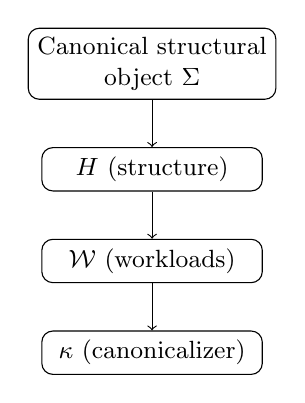
\begin{tikzpicture}[node distance=6mm, every node/.style={font=\small}]
    \node[draw, rounded corners, align=center, minimum width=2.8cm] (sig) {Canonical structural\\object $\Sigma$};
    \node[draw, rounded corners, align=center, below=of sig, minimum width=2.8cm] (H) {$H$ (structure)};
    \node[draw, rounded corners, align=center, below=of H, minimum width=2.8cm] (W) {$\mathcal W$ (workloads)};
    \node[draw, rounded corners, align=center, below=of W, minimum width=2.8cm] (k) {$\kappa$ (canonicalizer)};
    \draw[->] (sig) -- (H);
    \draw[->] (H) -- (W);
    \draw[->] (W) -- (k);
  \end{tikzpicture}
  \caption{The canonical structural object $\Sigma=(H,\mathcal W,\kappa)$ separates structure, workload space, and canonicalization.}
  \label{fig:canonical-object}
\end{figure}

\begin{figure}[t]
  \centering
  
\begin{tikzpicture}[node distance=6mm, every node/.style={font=\small}]
    \node[draw, rounded corners, align=center, minimum width=2.8cm] (Fd) {$F_d$};
    \node[draw, rounded corners, align=center, right=9mm of Fd, minimum width=2.8cm] (nu) {$\nu$};
    \node[draw, rounded corners, align=center, right=9mm of nu, minimum width=2.8cm] (kap) {$\kappa$};
    \node[draw, rounded corners, align=center, right=9mm of kap, minimum width=2.8cm] (P) {$P_\chi$};
    \node[draw, rounded corners, align=center, right=9mm of P, minimum width=2.8cm] (U) {$U$};
    \draw[->] (Fd) -- (nu);
    \draw[->] (nu) -- (kap);
    \draw[->] (kap) -- (P);
    \draw[->] (P) -- (U);
  \end{tikzpicture}
  \caption{Compilation stages in the structural compiler $C_\chi = U\circ P_\chi\circ\kappa\circ\nu\circ F_d$.}
  \label{fig:compilation-stages}
\end{figure}

\begin{figure}[t]
  \centering
  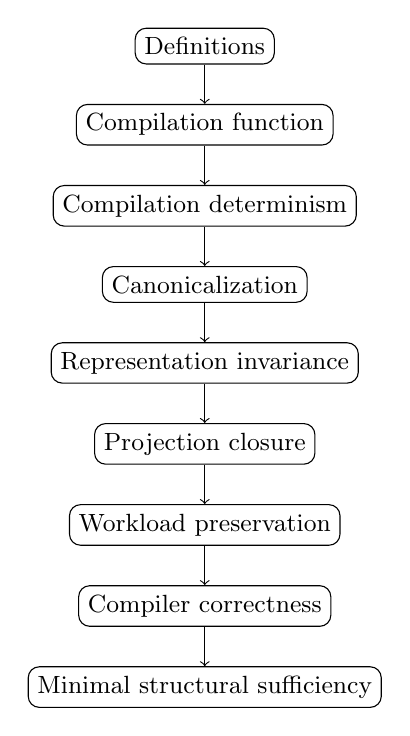
\begin{tikzpicture}[node distance=5mm, every node/.style={font=\small}]
    \node[draw, rounded corners, align=center] (defs) {Definitions};
    \node[draw, rounded corners, align=center, below=of defs] (comp) {Compilation function};
    \node[draw, rounded corners, align=center, below=of comp] (det) {Compilation determinism};
    \node[draw, rounded corners, align=center, below=of det] (can) {Canonicalization};
    \node[draw, rounded corners, align=center, below=of can] (inv) {Representation invariance};
    \node[draw, rounded corners, align=center, below=of inv] (proj) {Projection closure};
    \node[draw, rounded corners, align=center, below=of proj] (work) {Workload preservation};
    \node[draw, rounded corners, align=center, below=of work] (corr) {Compiler correctness};
    \node[draw, rounded corners, align=center, below=of corr] (min) {Minimal structural sufficiency};

    \draw[->] (defs) -- (comp);
    \draw[->] (comp) -- (det);
    \draw[->] (det) -- (can);
    \draw[->] (can) -- (inv);
    \draw[->] (inv) -- (proj);
    \draw[->] (proj) -- (work);
    \draw[->] (work) -- (corr);
    \draw[->] (corr) -- (min);
  \end{tikzpicture}
  \caption{Dependency structure of the main theorem chain.}
  \label{fig:theorem-deps}
\end{figure}
\paragraph{Theorem Dependency Summary.}
The logical dependencies among the principal results are summarized in Figure~\ref{fig:theorem-deps} and listed explicitly here as a verification aid.
\begin{itemize}[leftmargin=*]
  \item Theorem~\ref{thm:workload-preservation} (Workload Preservation) depends on Definition~\ref{def:canonical-structural-object} (canonical structural object) and the workload model (Section~\ref{sec:workload-model}).
  \item Theorem~\ref{thm:compilation-determinism} (Compilation Determinism) depends on Definition~\ref{def:compilation-function} (compilation function).
  \item Theorem~\ref{thm:canonicalization-idempotence} (Canonicalization Idempotence) depends on the canonical-normal-form assumption for $\kappa$.
  \item Theorem~\ref{thm:projection-closure} (Projection Closure) depends on Definition~\ref{def:counterfactual-deletion} (counterfactual deletion) and Definition~\ref{def:structural-equivalence} (structural equivalence).
  \item Theorem~\ref{thm:representation-invariance} (Representation Invariance) depends on Definition~\ref{def:structural-equivalence} (structural equivalence) and the canonicalization operator $\kappa$.
  \item Theorem~\ref{thm:compiler-correctness} (Compiler Correctness) depends on Theorems~\ref{thm:compilation-determinism}, \ref{thm:canonicalization-idempotence}, \ref{thm:projection-closure}, \ref{thm:workload-preservation}, and \ref{thm:representation-invariance}.
  \item Theorem~\ref{thm:minimal-structural-sufficiency} (Minimal Structural Sufficiency) depends on Definition~\ref{def:counterfactual-deletion}, Theorem~\ref{thm:representation-invariance}, and the deletion-and-reachability dependency predicate defined in Paper~1.
\end{itemize}

\section{Definitions}
\label{sec:definitions}
\paragraph{Notation.}
Let $\mathcal{D}$ denote a space of concrete system descriptions. Let $\mathcal{H}$ denote the class of finite structural graphs (Definition~\ref{def:structural-graph}). For a fixed workload class $\chi$, write $\mathcal{P}_\chi$ for the class of projected structural objects and $\mathcal{G}$ for the class of directed analysis graphs produced for downstream reachability-style queries.

\begin{definition}[System]
\label{def:system}
A \emph{system} is a finite executable structure (or process) presented via a concrete description $d\in\mathcal{D}$ such that there exists a deterministic extraction map $F_d$ producing a finite structural graph $H$ that is suitable for workload-relative analysis.
\end{definition}

\begin{definition}[Component]
\label{def:component}
A \emph{component} is a vertex $v\in V$ in a structural graph $H$ representing an indivisible unit of structure at the chosen abstraction level (e.g., a function, task, resource, dataset, service, or agent).
\end{definition}

\begin{definition}[Execution Relation]
\label{def:execution-relation}
An \emph{execution relation} is a directed edge $e=(u,v)\in E$ in a structural graph $H$ asserting that $u$ may directly enable, invoke, produce, trigger, or otherwise precede $v$ under the semantics of the source domain.
\end{definition}

\begin{definition}[Structural Graph]
\label{def:structural-graph}
A \emph{structural graph} is a finite typed attributed directed graph
\[
H=(V,E,\tau_V,\tau_E,\alpha),
\]
where $V$ is a finite set of components, $E\subseteq V\times V$ is a finite set of directed relations, $\tau_V:V\to\mathsf{T}_V$ and $\tau_E:E\to\mathsf{T}_E$ are typing maps, and $\alpha:(V\cup E)\to\mathsf{A}$ assigns finite structural attributes (e.g., labels, locations, or domain-specific metadata).
\end{definition}

\begin{definition}[Canonical Structural Object]
\label{def:canonical-structural-object}
A \emph{canonical structural object} is a triple
\[
\Sigma=(H,\mathcal{W},\kappa),
\]
where $H$ is a structural graph, $\mathcal{W}$ is a workload space over $H$, and $\kappa$ is a deterministic canonicalization operator.
\end{definition}

\begin{definition}[Counterfactual Deletion]
\label{def:counterfactual-deletion}
Let $H=(V,E,\tau_V,\tau_E,\alpha)$ be a structural graph and let $S\subseteq V$ be a designated candidate set. The \emph{counterfactual deletion} of $S$ from $H$ is the induced structural subgraph
\[
\pi_S(H)=H\upharpoonright_{V\setminus S},
\]
obtained by removing the vertices in $S$ and all incident edges.
\end{definition}

\begin{definition}[Compilation Function]
\label{def:compilation-function}
Fix a workload class $\chi$. A \emph{(structural) compilation function} is a map
\[
C_\chi = U\circ P_\chi\circ\kappa\circ\nu\circ F_d,
\]
where $F_d$ extracts a raw structural description from $d\in\mathcal{D}$, $\nu$ normalizes, $\kappa$ canonicalizes, $P_\chi$ projects to the information required by workload class $\chi$, and $U$ constructs the workload-specific directed graph used by later analyses.
\end{definition}

\section{Structural Graph Model}
\label{sec:structural-graph-model}
Having fixed the compilation interface (Definition~\ref{def:compilation-function}), we now specify the structural representation extracted from concrete systems.
We take the pre-workload compilation target to be the structural graph
\[
H=(V,E,\tau_V,\tau_E,\alpha)
\]
from Definition~\ref{def:structural-graph}. Here $V$ is the set of structural components, $E\subseteq V\times V$ is the set of directed structural relations, $\tau_V:V\to\mathsf{T}_V$ assigns a vertex type to each component, $\tau_E:E\to\mathsf{T}_E$ assigns an edge type to each relation, and $\alpha:(V\cup E)\to\mathsf{A}$ assigns (finite) structural attributes.

\section{Workload Model}
\label{sec:workload-model}
With the structural substrate fixed, we now make explicit the form of the queries (workloads) that will be posed against compiled objects.
A \emph{workload} is a query triple
\[
w=(R,t,S),
\]
where $R\subseteq V$ is a designated root set, $t\in V$ is a designated target, and $S\subseteq V$ is a designated candidate component set.

\begin{theorem}[Workload Preservation]
\label{thm:workload-preservation}
\deps{Definition~\ref{def:canonical-structural-object} (canonical structural object).}
Let $\Sigma=(H,\mathcal W,\kappa)$ be a canonical structural object (Definition~\ref{def:canonical-structural-object}).
Let $w=(R,t,S)\in\mathcal W$ be a workload on $H$, and let $P_\chi(H)$ be the workload-class projection of $H$.
Assume that $P_\chi$ maps the anchors $R$, $t$, and $S$ to well-defined images $R_\chi$, $t_\chi$, and $S_\chi$.
Then the projected workload $w_\chi=(R_\chi,t_\chi,S_\chi)$ is well defined on $P_\chi(H)$.
\end{theorem}
\begin{proof}
Assume the hypothesis that $P_\chi$ preserves the workload anchors.
Define $R_\chi:=P_\chi(R)$, $t_\chi:=P_\chi(t)$, and $S_\chi:=P_\chi(S)$.
Then $(R_\chi,t_\chi,S_\chi)$ is a well-formed workload triple over the projected object $P_\chi(H)$.
Therefore the projected workload $w_\chi$ is well defined on $P_\chi(H)$.
\end{proof}

\section{Canonical Structural Object}
\label{sec:canonical-structural-object}
Given a structural graph model, we take the principal object of study to be
\[
\Sigma=(H,\mathcal{W},\kappa),
\]
where $H$ is a structural graph, $\mathcal{W}\subseteq 2^V\times V\times 2^V$ is a workload space over $H$, and $\kappa$ is a deterministic map that identifies a canonical representative for each structural equivalence class.

\section{Compilation Function}
\label{sec:compilation-function}
Fix a workload class $\chi$. The structural compiler is the composition
\[
C_\chi = U\circ P_\chi\circ\kappa\circ\nu\circ F_d,
\]
with stages interpreted as follows: $F_d:\mathcal{D}\to\mathcal{H}$ (domain extraction), $\nu:\mathcal{H}\to\mathcal{H}$ (normalization), $\kappa:\mathcal{H}\to\mathcal{H}$ (canonicalization), $P_\chi:(\mathcal{H}\times\mathcal{W})\to\mathcal{P}_\chi$ (workload projection), and $U:\mathcal{P}_\chi\to\mathcal{G}$ (reachability-graph construction).

\subsection{Compilation Determinism}
\begin{theorem}[Compilation Determinism]
\label{thm:compilation-determinism}
\deps{Definition~\ref{def:compilation-function} (compilation function).}
Fix a workload class $\chi$ and let $C_\chi$ be the compilation function from Definition~\ref{def:compilation-function}.
Let $d\in\mathcal D$ be a concrete system description.
If the stages $F_d$, $\nu$, $\kappa$, $P_\chi$, and $U$ are deterministic, then the compiled output $C_\chi(d)$ is uniquely determined.
\end{theorem}
\begin{proof}
Assume $F_d$, $\nu$, $\kappa$, $P_\chi$, and $U$ are deterministic.
By Definition~\ref{def:compilation-function}, $C_\chi$ is their composition.
The composition of deterministic functions is deterministic, so the map $d\mapsto C_\chi(d)$ has a unique value for each input $d\in\mathcal D$.
Therefore $C_\chi(d)$ is uniquely determined.
\end{proof}


\section{Canonicalization}
\label{sec:canonicalization}

\begin{theorem}[Canonicalization Idempotence]
\label{thm:canonicalization-idempotence}
\deps{(Canonical normal form assumption for $\kappa$.)}
Let $H\in\mathcal H$ be a normalized structural graph.
If $\kappa$ maps every normalized structural object to a canonical normal form, then
\[
\kappa(\kappa(H))=\kappa(H).
\]
\end{theorem}
\begin{proof}
Assume $\kappa(H)$ is a canonical normal form representative for the structural equivalence class of $H$.
Then $\kappa(H)$ is already canonical, so re-applying $\kappa$ cannot change it without violating uniqueness of the canonical representative.
Therefore $\kappa(\kappa(H))=\kappa(H)$, establishing idempotence.
\end{proof}

\section{Projection Operators}
\label{sec:projection-operators}

Having defined canonicalization, we now state the key compatibility property between workload projection and counterfactual deletion.

\begin{theorem}[Projection Closure]
\label{thm:projection-closure}
\deps{Definition~\ref{def:counterfactual-deletion} (counterfactual deletion); Definition~\ref{def:structural-equivalence} (structural equivalence).}
Let $H=(V,E,\tau_V,\tau_E,\alpha)\in\mathcal H$ be a structural graph and let $S\subseteq V$.
Let $P_\chi$ denote workload-class projection.
Then projection commutes with counterfactual deletion (Definition~\ref{def:counterfactual-deletion}) up to structural equivalence (Definition~\ref{def:structural-equivalence}):
\[
P_\chi(\pi_S(H)) \equiv_{\mathrm{str}} \pi_S(P_\chi(H)).
\]
\end{theorem}
\begin{proof}
Assume a fixed workload class $\chi$.
By Definition~\ref{def:counterfactual-deletion}, $\pi_S(H)$ removes exactly the vertices in $S$ and their incident edges.
The projection $P_\chi$ removes exactly the structural information irrelevant to $\chi$.
Whether we delete $S$ first and then project, or project first and then delete the images of $S$, the surviving vertices and the $\chi$-relevant relations among them coincide.
Therefore the two resulting projected objects differ at most by representation artifacts (e.g., internal naming or ordering) and are structurally equivalent.
Hence $P_\chi(\pi_S(H)) \equiv_{\mathrm{str}} \pi_S(P_\chi(H))$.
\end{proof}
\section{Structural Equivalence}
\label{sec:structural-equivalence}

Later results (notably Representation Invariance, Theorem~\ref{thm:representation-invariance}) use an equivalence relation that identifies structural objects differing only by representation artifacts such as naming, ordering, or serialization choices. We now make that relation explicit.

\begin{definition}[Structural Equivalence]
\label{def:structural-equivalence}
Let
\(H_i=(V_i,E_i,\tau^i_V,\tau^i_E,\alpha_i)\) for \(i\in\{1,2\}\) be structural graphs.
We say \(H_1\) and \(H_2\) are \emph{structurally equivalent}, written
\[
H_1 \equiv_{\mathrm{str}} H_2,
\]
if there exists a bijection \(\varphi:V_1\to V_2\) such that:
\begin{enumerate}[label=(\roman*),leftmargin=*]
  \item \textbf{Edge preservation:} \((u,v)\in E_1\) iff \((\varphi(u),\varphi(v))\in E_2\).
  \item \textbf{Type preservation:} for all \(u\in V_1\), \(\tau^1_V(u)=\tau^2_V(\varphi(u))\); and for all \((u,v)\in E_1\),
  \(\tau^1_E(u,v)=\tau^2_E(\varphi(u),\varphi(v))\).
  \item \textbf{Attribute agreement up to artifacts:} for all \(x\in V_1\cup E_1\),
  \(\alpha_1(x)\) and \(\alpha_2(\varphi(x))\) agree on all \emph{semantic} attributes required by the workload class under study (and may differ on representation artifacts such as internal identifiers, storage addresses, or ordering metadata).
\end{enumerate}
\end{definition}

\noindent The third condition intentionally treats ``semantic'' vs.
``artifact'' attributes as a design choice fixed by the domain and workload class; canonicalization $\kappa$ is required to erase the artifact portion deterministically.

\section{Representation Invariance}
\label{sec:representation-invariance}

\begin{theorem}[Representation Invariance]
\label{thm:representation-invariance}
\deps{Definition~\ref{def:structural-equivalence} (structural equivalence).}
Let $H_1,H_2\in\mathcal H$ be normalized structural graphs.
If $H_1 \equiv_{\mathrm{str}} H_2$ (Definition~\ref{def:structural-equivalence}), then $\kappa(H_1)=\kappa(H_2)$.
\end{theorem}
\begin{proof}
Assume $H_1 \equiv_{\mathrm{str}} H_2$.
By Definition~\ref{def:structural-equivalence}, $H_1$ and $H_2$ agree on all semantic structure relevant to the chosen workload class and may differ only by representation artifacts.
By construction, canonicalization $\kappa$ deterministically erases those artifacts and selects a unique canonical representative for each structural equivalence class.
Therefore $\kappa(H_1)$ and $\kappa(H_2)$ are the same representative, i.e., $\kappa(H_1)=\kappa(H_2)$.
\end{proof}

% Theorem~\ref{thm:compiler-correctness} is the main end-to-end guarantee of the compilation contract.
\medskip
\noindent\textbf{Central guarantee.} The following theorem packages the stage-level contracts into a single statement: if each stage satisfies its invariants, then dependency answers (Paper~1) are invariant under structural equivalence.

\begin{theorem}[Compiler Correctness]
\label{thm:compiler-correctness}
\deps{Definition~\ref{def:compilation-function}; Theorems~\ref{thm:compilation-determinism}, \ref{thm:canonicalization-idempotence}, \ref{thm:projection-closure}, \ref{thm:workload-preservation}, \ref{thm:representation-invariance}.}
Fix a workload class $\chi$ and let $C_\chi$ be the compilation function from Definition~\ref{def:compilation-function}.
Let $d\in\mathcal D$ be a concrete system description and write
\[
C_\chi(d)=(G,w)
\]
for the compiled analysis graph and induced workload anchors.
If the compiler satisfies:
\begin{enumerate}[label=(\roman*),leftmargin=*]
    \item Compilation Determinism (Theorem~\ref{thm:compilation-determinism}),
    \item Canonicalization Idempotence (Theorem~\ref{thm:canonicalization-idempotence}),
    \item Projection Closure (Theorem~\ref{thm:projection-closure}),
    \item Workload Preservation (Theorem~\ref{thm:workload-preservation}), and
    \item Representation Invariance (Theorem~\ref{thm:representation-invariance}),
\end{enumerate}
then every dependency query evaluated on $(G,w)$ is representation-independent with respect to the structural equivalence relation $\equiv_{\mathrm{str}}$.
\end{theorem}
\begin{proof}
Assume conditions (i)--(v).
By Theorem~\ref{thm:compilation-determinism}, the pipeline output is uniquely determined for each input description $d$; in particular, no stage-level nondeterminism can change the compiled analysis instance $(G,w)$.
By Theorem~\ref{thm:representation-invariance}, any two structurally equivalent normalized inputs are mapped by $\kappa$ to the same canonical representative, so representation artifacts cannot change the canonical structural content that is passed downstream.
By Theorem~\ref{thm:canonicalization-idempotence}, once the canonical representative is reached it is stable under re-canonicalization, so repeated compilation/canonicalization cannot introduce drift.
By Theorem~\ref{thm:projection-closure}, counterfactual deletion (of candidate components) and workload projection commute up to $\equiv_{\mathrm{str}}$, so the order in which we (i) form the workload-specific view and (ii) apply the Paper~1 deletion operation does not affect the projected structural content relevant to reachability.
By Theorem~\ref{thm:workload-preservation}, the workload anchors (roots, target, candidate set) are mapped consistently into the projected object on which $G$ is constructed, so the query instance is well posed.
Therefore the dependency predicate of Paper~1, when evaluated on $(G,w)$, depends only on canonical structural content and not on naming, ordering, or other representation artifacts.
Hence dependency answers are representation-independent with respect to $\equiv_{\mathrm{str}}$.
\end{proof}

\begin{theorem}[Minimal Structural Sufficiency]
\label{thm:minimal-structural-sufficiency}
\deps{Definition~\ref{def:counterfactual-deletion} (deletion); Theorem~\ref{thm:representation-invariance} (invariance).}
Let $d\in\mathcal D$ and let $C_\chi(d)=(G,w)$.
If the compilation pipeline preserves (i) path fidelity, (ii) deletion fidelity (Definition~\ref{def:counterfactual-deletion}), (iii) workload-anchor fidelity, and (iv) representation invariance (Theorem~\ref{thm:representation-invariance}),
then $G$ contains sufficient structural information to evaluate every workload-relative dependency query in the class $\chi$.
\end{theorem}
\begin{proof}
Assume the stated fidelity properties.
Path fidelity ensures that directed reachability in $G$ corresponds to admissible structural paths in the underlying system.
Deletion fidelity (via counterfactual deletion, Definition~\ref{def:counterfactual-deletion}) ensures that removing candidate components in the system corresponds to deleting the associated vertices/edges in $G$.
Workload-anchor fidelity ensures that roots, targets, and candidate sets in $w$ refer to the intended vertices in $G$.
Finally, representation invariance ensures these correspondences do not depend on naming, ordering, or other incidental representation artifacts.
Therefore $G$ contains exactly the information needed to apply deletion-and-reachability dependency queries for workload class $\chi$.
\end{proof}

\section{Complexity Analysis}
\label{sec:complexity}

Let $d$ be a concrete system description and let
\[
H=(V,E,\tau_V,\tau_E,\alpha)
\]
be the extracted structural graph. Let
\[
G_\chi=(V_\chi,E_\chi)
\]
be the workload-class reachability graph produced after projection. We analyze costs in terms of
\[
|d|,\ |V|,\ |E|,\ |V_\chi|,\ |E_\chi|,\ |R|,\ |S|.
\]

The framework separates the cost of constructing a canonical structural object from the cost of evaluating a dependency query on a projected graph.

\paragraph{Stage costs.}
Assume adjacency-list representations for $H$ and $G_\chi$.
\begin{enumerate}[label=(\roman*),leftmargin=*]
    \item \textbf{Domain extraction $F_d$:} domain-dependent; at minimum $\Omega(|d|)$.
    \item \textbf{Normalization $\nu$:} $O(|V|+|E|)$.
    \item \textbf{Canonicalization $\kappa$:} write $C_\kappa(H)$ for the canonicalization cost on $H$.
    A common deterministic strategy (e.g., sorting vertices/edges for stable serialization) is
    \[
    O\bigl((|V|+|E|)\log(|V|+|E|)\bigr),
    \]
    while stronger forms (e.g., canonical labeling up to isomorphism) may be more expensive in the worst case and are intentionally not collapsed into a single polynomial claim.
    \item \textbf{Workload projection $P_\chi$:} $O(|V|+|E|)$.
    \item \textbf{Reachability-graph construction $U$:} $O(|V_\chi|+|E_\chi|)$.
\end{enumerate}

\paragraph{Query costs on $G_\chi$.}
For a workload $w_\chi=(R_\chi,t_\chi,S_\chi)$ on $G_\chi$:
\begin{enumerate}[label=(\roman*),leftmargin=*]
    \item \textbf{Deletion $\pi_S$:} $O(|V_\chi|+|E_\chi|)$, e.g., by filtering to active vertices and incident edges.
    \item \textbf{Reachability $\rho$:} $O(|V_\chi|+|E_\chi|)$ via BFS/DFS.
\end{enumerate}
Consequently, the total cost of a single dependency query after compilation is
\[
O(|V_\chi|+|E_\chi|).
\]

\paragraph{End-to-end bound.}
A conservative end-to-end bound for producing $G_\chi$ from $d$ and then answering one dependency query is
\[
O\bigl(|d| + C_\kappa(H) + |V| + |E| + |V_\chi| + |E_\chi|\bigr).
\]

\section{Discussion}
\label{sec:discussion}

% [Audit: Citation optional] High-level framing of implications.
The technical development above defines an interface between two kinds of objects: (i) heterogeneous, domain-specific system descriptions, and (ii) workload-relative predicates (Paper~1) that require a directed analysis graph and a consistent notion of counterfactual deletion. Making that interface explicit has several implications.

% [Audit: No citation needed] Original consequence statements (enabled analyses) built from this paper's framework.
\paragraph{What the framework enables.}
Once a domain admits a front end $F_d$ into a typed structural graph $H$, later analyses can be expressed as workload-class projections and graph queries on $G_\chi=U(P_\chi(\kappa(\nu(F_d(d)))))$. This includes, beyond workload-relative dependency (Paper~1):
\begin{enumerate}[label=(\roman*),leftmargin=*]
  \item \textbf{Resilience analysis:} quantify how dependency answers change under removal of components or relations, and identify minimal cut sets or ``single points of failure'' relative to a workload class.
  \item \textbf{Redundancy analysis:} detect multiple disjoint structural witnesses for reachability and characterize when dependency is robust to counterfactual deletions.
  \item \textbf{Counterfactual analysis:} compare worlds produced by families of deletions (or hypothetical additions), using $\kappa$ to factor out representational variation.
  \item \textbf{Optimization and refactoring:} treat $\kappa$ and $P_\chi$ as contracts that allow refactorings or compilation changes while preserving workload answers.
  \item \textbf{Governance and accountability:} when systems are socio-technical, canonical structural objects provide a stable substrate for auditing and policy reasoning (e.g., continuity-oriented governance layers).
\end{enumerate}

% [Audit: No citation needed] Interpretation of this paper's modeling choice.
\paragraph{Interpretation of canonicalization.}
Canonicalization $\kappa$ should not be interpreted as claiming a single universal representation across domains; different domains may instantiate $\kappa$ differently while preserving the same compiler contract. Rather, it enforces a deterministic choice of representative within a domain- and workload-appropriate structural equivalence class (Definition~\ref{def:structural-equivalence}). This shifts debates about ``the right graph'' into explicit modeling choices: which attributes are semantic for a workload class, and which are artifacts that must not influence answers.

% [Audit: Citation required] Claims about implementability using existing infrastructures.
\paragraph{Relationship to existing IR and provenance tooling.}
Because the framework is staged, it can be implemented using existing compiler IR infrastructure (for software) \cite{llvmLangRef,mlirDoc} or provenance/workflow graph infrastructure (for data systems) \cite{w3cprov,deelman2009}, while still enforcing the invariants required for representation-independent downstream queries.

\section{Limitations}
\label{sec:limitations}

\paragraph{Equivalence is workload- and domain-relative.}
Structural equivalence (Definition~\ref{def:structural-equivalence}) depends on what counts as a semantic attribute for a given workload class. Different choices can change both the strength of representation invariance and the feasibility/cost of $\kappa$.

\paragraph{Canonicalization may be expensive in the worst case.}
While many practical settings admit light-weight deterministic canonicalization (e.g., stable serialization), stronger invariance goals can approach canonical labeling complexity. The framework isolates this cost (Section~\ref{sec:complexity}) but does not remove it.

\paragraph{Front-end assumptions.}
The framework assumes a deterministic extraction function $F_d$. In practice, extraction may depend on dynamic execution, environment configuration, or incomplete specifications; such settings require either enriched system descriptions or probabilistic/parametric structural objects.

\paragraph{Projection can be lossy.}
Workload projection $P_\chi$ is intentionally selective. If a later analysis needs information not preserved by the chosen projection, the projection contract must be strengthened (or multiple projections must coexist).

\section{Future Work}
\label{sec:future-work}

Several extensions are natural.
\begin{enumerate}[label=(\roman*),leftmargin=*]
  \item \textbf{Domain instantiations and case studies:} define concrete $F_d,\nu,\kappa,P_\chi$ for at least one compiler domain (e.g., LLVM/MLIR) and one provenance/workflow domain (e.g., W3C PROV-style graphs), and empirically evaluate invariance and cost.
  \item \textbf{Richer structural equivalences:} study families of $\equiv_{\mathrm{str}}$ that incorporate attribute abstractions, partial observability, or semantic equivalences stronger than graph isomorphism.
  \item \textbf{Incremental and streaming compilation:} support evolving systems by maintaining $\kappa(H)$ and $G_\chi$ under updates, enabling continuous dependency and resilience monitoring.
  \item \textbf{Query languages and tool support:} expose workload classes and projections through a declarative interface so that analyses can be authored without hard-coding domain-specific graph transformations.
  \item \textbf{Governance layers:} connect canonical structural objects to policy and continuity governance artifacts to make accountability constraints first-class alongside technical dependency queries.
\end{enumerate}
\section{Conclusion}
\label{sec:conclusion}

Paper~1 formalized workload-relative dependency as a predicate computed by counterfactual deletion and reachability on a directed analysis graph.
This paper addressed the missing prior question: given a heterogeneous concrete system description, what exactly is the graph on which that predicate operates?

We answered by defining a deterministic structural compilation contract $C_\chi=U\circ P_\chi\circ\kappa\circ\nu\circ F_d$ that produces a workload-class analysis graph (and consistent workload anchors) in a representation-independent way.
Together, Papers~1 and~2 establish a mathematical foundation for workload-relative structural analysis in which downstream results depend on canonical structural content rather than incidental representation artifacts.
In particular, Theorem~\ref{thm:compiler-correctness} establishes representation-independent dependency answers for compiled instances, and Theorem~\ref{thm:minimal-structural-sufficiency} establishes that the compiled analysis graph contains sufficient information to evaluate dependency queries in the workload class.

With the dependency predicate and its compilation target fixed, subsequent papers can focus on analyses enabled by this foundation---including dependency analysis at scale (Paper~1), and extensions such as resilience, redundancy, counterfactual, optimization, and governance-oriented reasoning built on top of canonical structural objects.
\appendix

\section{Notation (alphabetical)}
\label{app:notation}
\begin{table}[h]
\centering
\begin{tabular}{@{}ll@{}}
\toprule
Symbol & Meaning \\
\midrule
$C_\chi$ & Structural compilation function for workload class $\chi$ (Definition~\ref{def:compilation-function}) \\
$d\in\mathcal D$ & Concrete system description / description space \\
$E$ & Edge set of a structural graph $H$ \\
$F_d$ & Domain extraction / front end (Section~\ref{sec:compilation-function}) \\
$G_\chi$ & Workload-class directed analysis graph produced after projection \\
$H$ & Structural graph (Definition~\ref{def:structural-graph}) \\
$P_\chi$ & Workload-class projection operator (Section~\ref{sec:compilation-function}) \\
$R,t,S$ & Workload anchors: roots, target, candidate set (Section~\ref{sec:workload-model}) \\
$U$ & Reachability-graph construction stage (Section~\ref{sec:compilation-function}) \\
$V$ & Vertex set (components) of a structural graph $H$ \\
$w=(R,t,S)$ & Workload/query triple (Section~\ref{sec:workload-model}) \\
$\alpha$ & Attribute map of a structural graph $H$ (Definition~\ref{def:structural-graph}) \\
$\equiv_{\mathrm{str}}$ & Structural equivalence relation (Definition~\ref{def:structural-equivalence}) \\
$\kappa$ & Canonicalization operator (Definition~\ref{def:canonical-structural-object}) \\
$\mathcal W$ & Workload space over $H$ (Definition~\ref{def:canonical-structural-object}) \\
$\nu$ & Normalization stage (Section~\ref{sec:compilation-function}) \\
$\pi_S(H)$ & Counterfactual deletion of $S$ from $H$ (Definition~\ref{def:counterfactual-deletion}) \\
$\Sigma$ & Canonical structural object $(H,\mathcal W,\kappa)$ (Definition~\ref{def:canonical-structural-object}) \\
$\tau_V,\tau_E$ & Vertex/edge typing maps of $H$ (Definition~\ref{def:structural-graph}) \\
\bottomrule
\end{tabular}
\caption{Core notation used throughout the manuscript, alphabetized by symbol.}
\end{table}

\section{Appendix A}
\label{app:a}

\section{Appendix B}
\label{app:b}

\bibliographystyle{plain}
\bibliography{references}

\end{document}
